\documentclass{article}
\usepackage[utf8]{inputenc}
\usepackage[a4paper, total={6in, 8in}]{geometry}

\usepackage[normalem]{ulem}
\usepackage{graphicx}
\usepackage{float}

\graphicspath{ {./images/} }

\title{CPSC 410 Notes}
\author{Kaitian Xie}
\date{June 2020}

\begin{document}

\maketitle
\pagebreak

\tableofcontents
\pagebreak

\section{Learning Objectives}

\begin{itemize}
    \item Domain Specific Languages (DSLs)
    \begin{enumerate}
        \item \sout{Differentiate Domain Specific Languages (DSLs) from general-purpose programming languages and libraries, and motivate their usefulness.}
        \item \sout{Design a DSL tailored to assist a target kind of user with specific task.}
        \item \sout{Implement a DSL simply, providing clear and suitably-robust error handling.}
        \item \sout{Evaluate a language design's effectiveness via user studies, and incorporate user feedback by processing revisions to a language design.}
        \item \sout{Compare DSL motivations and justify which you find appropriate (or not).}
        \item \sout{Judge how useful you find a particular DSL design for a given task/user, identifying and estimating the significance of any weaknesses.}
        \item Describe the key stages of a typical DSL implementation, including their roles.
        \item Explain trade-offs regarding whether to have particular phases do more or less work (e.g. fine-grained tokenization, grammar precision, validation).
        \item Propose a suitable tokenization for given input examples in a given language.
        \item Design a corresponding grammar for a given language and tokenization.
        \item Summarise the example tokenization/parsing strategies from the lectures, identifying their advantages and concrete limitations; mention alternatives.
        \item Justify the significance of specific language design principles.
        \item Give examples of considerations that API and designers should be aware of.
        \item Evaluate language features and designs against the language design principles we've discussed in the course, applying your own judgement.
        \item Design and run user studies to evaluate design questions empirically.
        \item Reflect on user feedback to identify potential root causes of any difficulties.
        \item Address these root problems with appropriate redesign ideas.
        \item \sout{Implement evaluation methods for an AST (or similar data structures)}.
        \item Contrast the two evaluation approaches here (AST methods vs. Visitors).
        \item Judge when AST functionality should be refactored using the Visitor Pattern.
        \item Explain how the Visitor pattern simulates double-dispatch, and why double dispatch is important for the user (and reuse) of the pattern.
        \item \sout{Choose when to use appropriate extensions of the underlying design patterns.}
        \item Give examples of a variety of attributes that may be bound to identifiers.
        \item Differentiate between attributes which are statically and dynamically bound.
        \item Implement language support for standard variable operations.
        \item Select appropriate representations for states used during evaluation.
        \item Illustrate the difference that aliasing makes to observable program behaviours, as well as on the necessary complexity of states used during evaluation.
        \item Contrast the trade-offs between static and dynamic checking, identifying the consequences of each (or neither) for users and language implementers.
        \item Justify whether a correctness property can be checked statically/dynamically.
        \item Implement static and dynamic checkers for particular correctness properties.
        \item Design test cases to illustrate relevant corner cases for a correctness property.
    \end{enumerate}
    \item User-Driven Language Design and Empirical Studies
    \begin{enumerate}
        \setcounter{enumi}{31}
        \item Compare user-centric design (particularly for teaching) with language design in general, giving example motivations for user-centric languages (Logo, Grace) and how their motivations influenced their designs specifically.
        \item Design ethical empirical studies, appropriately identifying risks (and their importance) and strategies for mitigating risks when possible.
        \item Evaluate empirical studies for threats to validity, judge their likely impact on a study's conclusion, and propose strategies for mitigating these when possible.
    \end{enumerate}
    \item Program Analysis and Visualization
    \begin{enumerate}
        \setcounter{enumi}{34}
        \item Differentiate the main types of program analysis, comparing their potential applications, strengths, and weaknesses.
        \item \sout{Design program analyses to extract and synthesise information to aid programmers with their daily work.}
        \item \sout{Implement simple program analyses and visualizations of their results.}
        \item \sout{Create useful visualizations of programming-related data.}
        \item \sout{Justify the likely usefulness of program analyses and visualizations.}
        \item \sout{Evaluate particular program analyses/visualizations using empirical studies.}
        \item Categorise analyses according to the main types presented here, justifying which are necessary/useful for which tasks.
        \item Contrast the pros and cons of raw-data vs. static program analyses, in situations where either could be applicable.
        \item Describe the high-level implementation strategies for making large-scale static/meta-property analyses efficient.
        \item Justify which properties about code a value-agnostic static analysis can be used for (or cannot be used for).
        \item Provide examples of key main points for value-agnostic static analyses.
        \item Define the notion of all-executions properties, giving examples.
        \item Explain the key ideas of the Static Program Slicing technique presented here.
        \item Apply the Static Program Slicing technique to produce program slices for simple imperative programs.
        \item Explain the causes of approximation for static program analyses, giving examples.
        \item Contrast dynamic program analyses with their static counterparts, explaining the typical trade-offs.
        \item Contrast the pros and cons of the main implementation methods for dynamic program analyses (when instrumentation is performed).
        \item Apply the Dynamic Program Slicing technique to produce program slices for simple imperative programs.
        \item Explain the concepts of over- and under-approximation, and their practical consequences for the analysis of correctness properties.
        \item Derive appropriate Failure Conditions for given statements and correctness properties of interest.
        \item Define the key ideas of the symbolic execution techniques presented here, and their meanings in the context of checking correctness properties.
        \item Apply the symbolic execution technique to simple imperative programs.
        \item Justify which of the standard pain points for a program analysis are addressed by symbolic execution (and which are not).
    \end{enumerate}
    \item Digesting and Evaluating PL/SE Research Papers
    \begin{enumerate}
        \setcounter{enumi}{57}
        \item Explain the key things to look for when skim-reading a research paper.
        \item \sout{Apply your knowledge of empirical evaluation techniques to critically evaluate the evidence provided in a research paper.}
        \item \sout{Create short, high-level, summaries of the main points of a research paper.}
    \end{enumerate}
\end{itemize}

\section{Domain Specific Languages}

\subsection{EBNF}

\begin{itemize}
    \item Examples
    \begin{itemize}
        \item L2 (13)
        \item L2 (15)
        \item A1 (2)
        \item A1 (3)
        \item A1 (4)
        \item A1 (5)
    \end{itemize}
\end{itemize}

\subsection{Tokenization and Parsing Strategies}

\begin{itemize}
    \item Tokenization
    \begin{itemize}
        \item Process
            \begin{itemize}
                \item Pick ``\_'' as a reserved word.
                \item Read the entire program as a string without new lines.
                \item Replace all constant literals with ``\_$<$literal$>$\_''.
                \item Replace ``\_\_'' with ``\_''.
                \item Split on ``\_''.
                \item (If needed) pattern matches for non-constant literals during parsing.
            \end{itemize}
        \item Examples
            \begin{itemize}
                \item Tokenizer.java
            \end{itemize}
    \end{itemize}
    \item Parsing
    \begin{itemize}
        \item Define the ``parse'' method of each node.
        \begin{itemize}
            \item Check the next token.
            \item Create a child node for a sub-statement.
            \item Parse on child nodes before continuing (recursive descent parsing).
        \end{itemize}
        \item Or do the parsing separately from the AST.
        \item Examples
        \begin{itemize}
            \item tinyHTML
            \item tinyDotStarter-parsingCompleted
        \end{itemize}
    \end{itemize}
\end{itemize}

\subsection{Key Stages of DSL Implementation}

\begin{itemize}
    \item Tokenize
    \begin{itemize}
        \item Split your input into basic elements from your syntax.
    \end{itemize}
    \item Parse
    \begin{itemize}
        \item Check your syntax and build an internal representation (AST).
    \end{itemize}
    \item {[Validate]}
    \begin{itemize}
        \item Enforce desired correctness properties for allowed programs (e.g. types).
    \end{itemize}
    \item Evaluate
    \begin{itemize}
        \item Execute program directly (DSL interpreter), or generate code to be run externally (DSL compiler).
    \end{itemize}
\end{itemize}

Example: L2 (5-13)

\subsection{Recursive Evaluation and Visitor Pattern}

\begin{itemize}
    \item Recursive Evaluation
    \begin{itemize}
        \item Process
        \begin{itemize}
            \item Start at the root of the AST.
            \item Carry out the work needed by the current node.
            \item Call ``evaluate'' recursively on all child nodes.
            \item Get the output by returning a value, modifying an existing object, printing, etc.
        \end{itemize}
        \item Examples
        \begin{itemize}
            \item tinyHTML
            \item tinyDotStarter-evaluationCompleted
        \end{itemize}
    \end{itemize}
    \item Visitor Pattern
    \begin{itemize}
        \item
        \begin{minipage}{\linewidth}
            \centering
            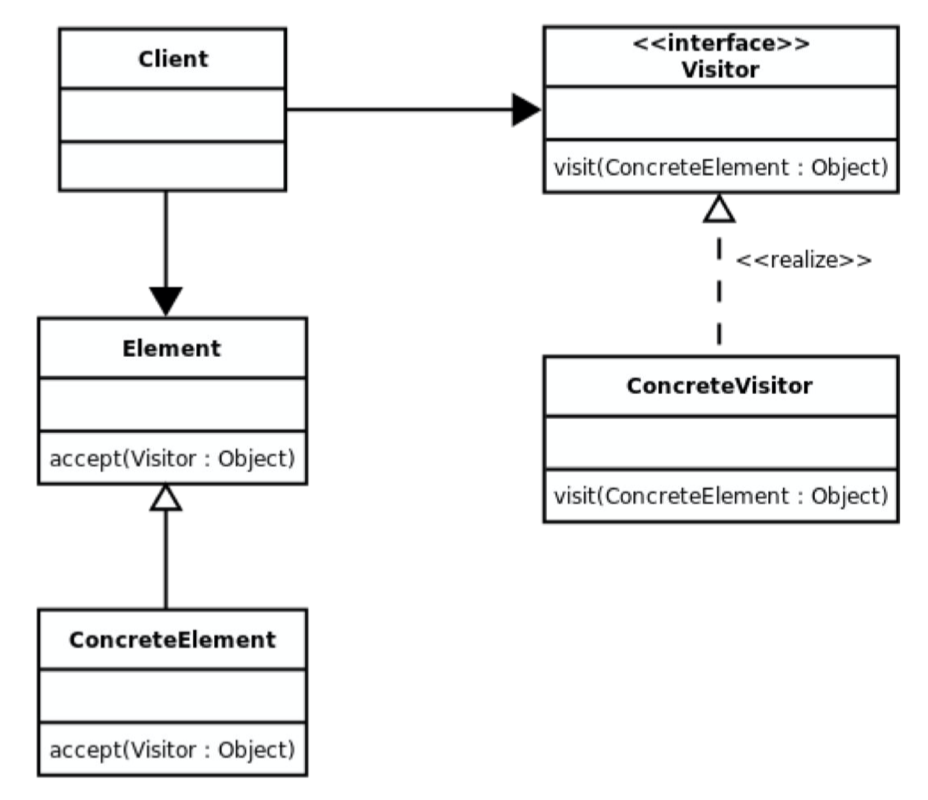
\includegraphics[width=\textwidth]{visitor_pattern}
        \end{minipage}
        \item Defines external functionality over ASTs.
        \item Useful for refactoring ASTs.
        \begin{itemize}
            \item Supports multiple kinds of evaluation.
            \item Separates AST evaluation from AST representation.
            \item Prevents violation against the Single Responsibility Principle.
        \end{itemize}
        \item Examples
        \begin{itemize}
            \item tinyDotStarter-Visitor
            \item tinyVars-Visitor
        \end{itemize}
    \end{itemize}
\end{itemize}

\subsection{Visitor Pattern and Double Dispatch}

\begin{itemize}
    \item Single dispatch: methods are dispatched based on the dynamic type of a single object (the receiver in Java).
    \item Visitor Pattern uses two single-dispatched method to simulate double dispatch (L4 (15-17)).
    \begin{itemize}
        \item Every subclass of Node has an ``accept'' method.
        \item A call to the ``accept'' method is dynamically dispatched to the subclass, where the static type of ``this'' is the same as the dynamic type of ``this'' object.
        \item The we use it to select the indented (overloaded) ``visit'' method.
    \end{itemize}
    \item Double dispatch is important for code reuse.
    \begin{itemize}
        \item No need to change the code that represents ASTs.
        \item Easy to implement different visitors that make use of the ASTs for different purposes.
    \end{itemize}
\end{itemize}

\subsection{Attributes}

\begin{itemize}
    \item Properties of a named program element.
    \begin{itemize}
        \item Name.
        \item Fact that it's a variable.
        \item Declaration site.
        \item Scope.
        \item Initialization status.
        \item Declared type.
        \item Current value.
        \item Location in memory.
    \end{itemize}
\end{itemize}

\subsection{Binding}

\begin{itemize}
    \item Associates attributes with names.
    \item Static (statically bound): known at/before compile time.
    \begin{itemize}
        \item Declared variable types.
        \item Selecting between overloaded methods for a call.
    \end{itemize}
    \item Dynamic (dynamically bound): chosen only at runtime.
    \begin{itemize}
        \item Calling overridden methods.
        \item Variable values.
    \end{itemize}
\end{itemize}

\subsection{Implementation of TinyVars}

\begin{itemize}
    \item L5 (11-26)
    \item tinyVars-UndefAlias
\end{itemize}

\subsection{What Could Be Checked Statically/Dynamically?}

\begin{figure}[H]
    \centering
    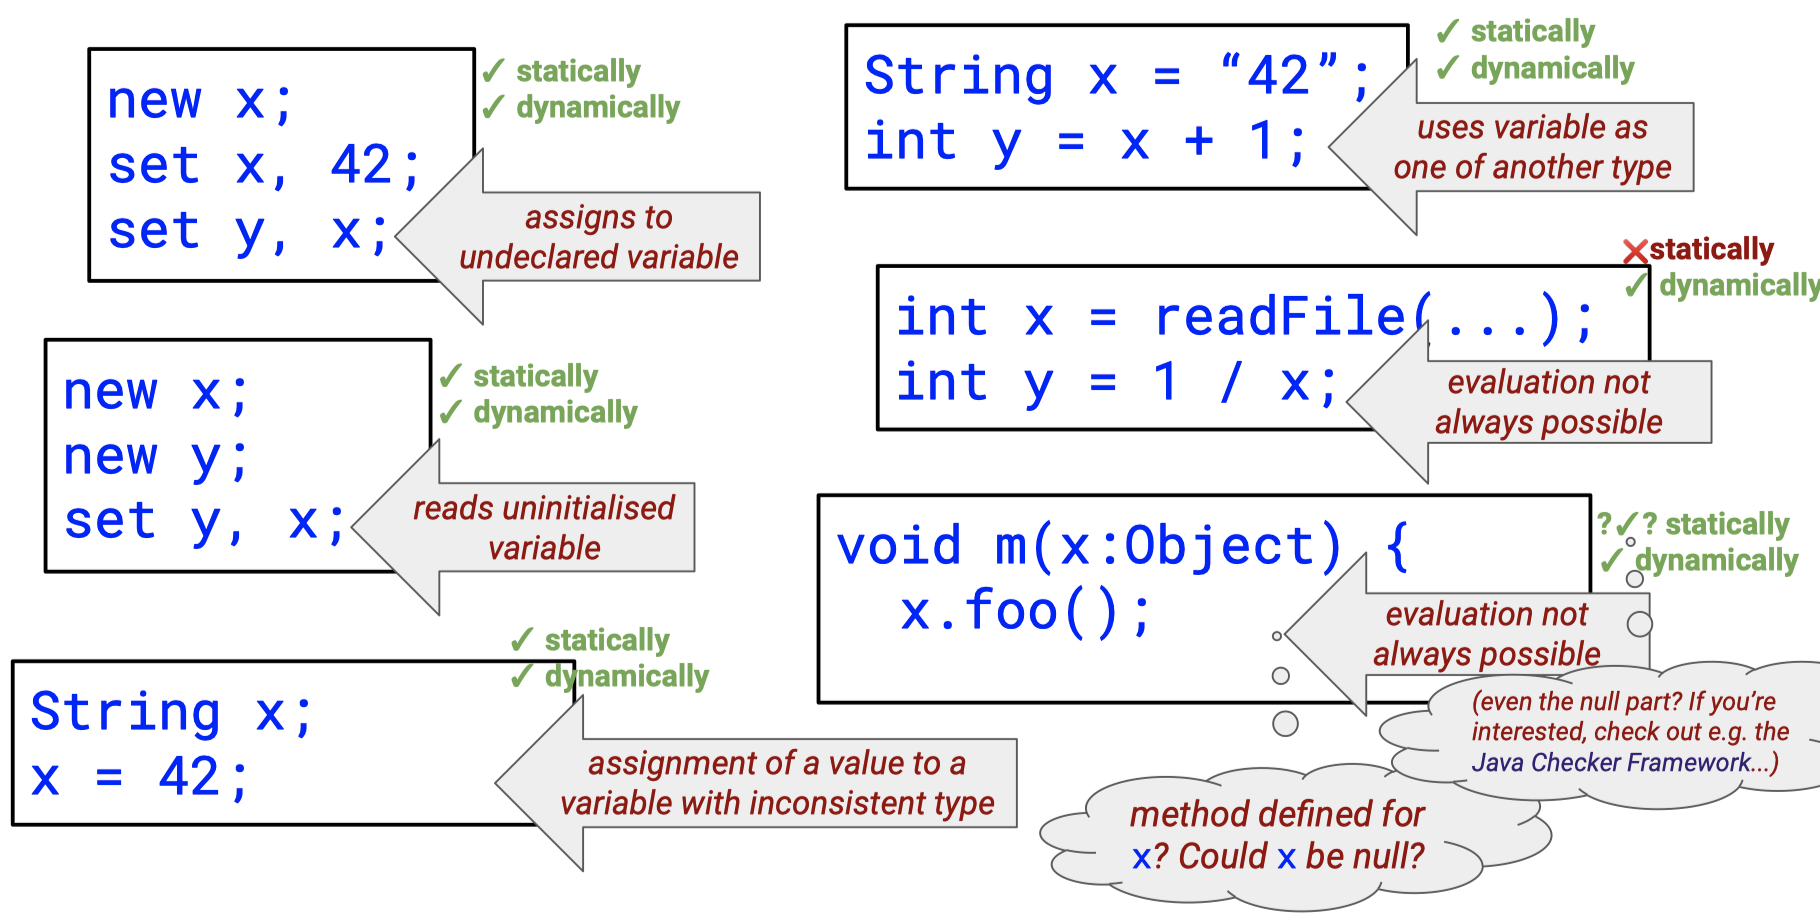
\includegraphics[width=\textwidth]{what_could_be_checked}
\end{figure}

\begin{itemize}
    \item A property in terms of dynamically-bound attributes cannot be checked statically
    \item A property that can be checked dynamically must have relevant attributes present at runtime.
\end{itemize}

\subsection{Static vs. Dynamic Checking}

\begin{itemize}
    \item Static Checking
    \begin{itemize}
        \item Checks enforced at/before compile time.
        \item Only possible for properties in terms of statically-bound attributes.
        \item Implemented via a traversal of the AST (e.g. with a visitor).
        \item Can justify simpler/more efficient program evaluation (properties can be assumed).
    \end{itemize}
    \item Dynamic Checking
    \begin{itemize}
        \item Checks at runtime.
        \item Properties may depend on attributes bound statically/dynamically (or both).
        \item Can check more flexible properties (e.g. changing variable types at runtime).
        \item Info must be present at runtime.
        \item Maybe slow.
    \end{itemize}
\end{itemize}

\subsection{Implementation of Static/Dynamic Checking}

\begin{itemize}
    \item Check options
    \begin{itemize}
        \item Check and complain.
        \item Check and adapt.
        \item Ignore.
    \end{itemize}
    \item Use the Visitor Pattern to implement the checking.
    \begin{itemize}
        \item Use ``String'' as return type.
        \begin{itemize}
            \item Empty string $\rightarrow$ no error.
            \item Otherwise $\rightarrow$ error message.
        \end{itemize}
        \item Use a ``Set$<$String$>$'' parameter to keep track of currently declared variables.
    \end{itemize}
    \item Examples
    \begin{itemize}
        \item tinyVars-StaticChecks
    \end{itemize}
\end{itemize}

\section{User-Driven Language Design and Empirical Studies}

\subsection{Logo and Grace}

L7 (5-13)

\subsection{The Empirical Method}

\begin{figure}[H]
    \centering
    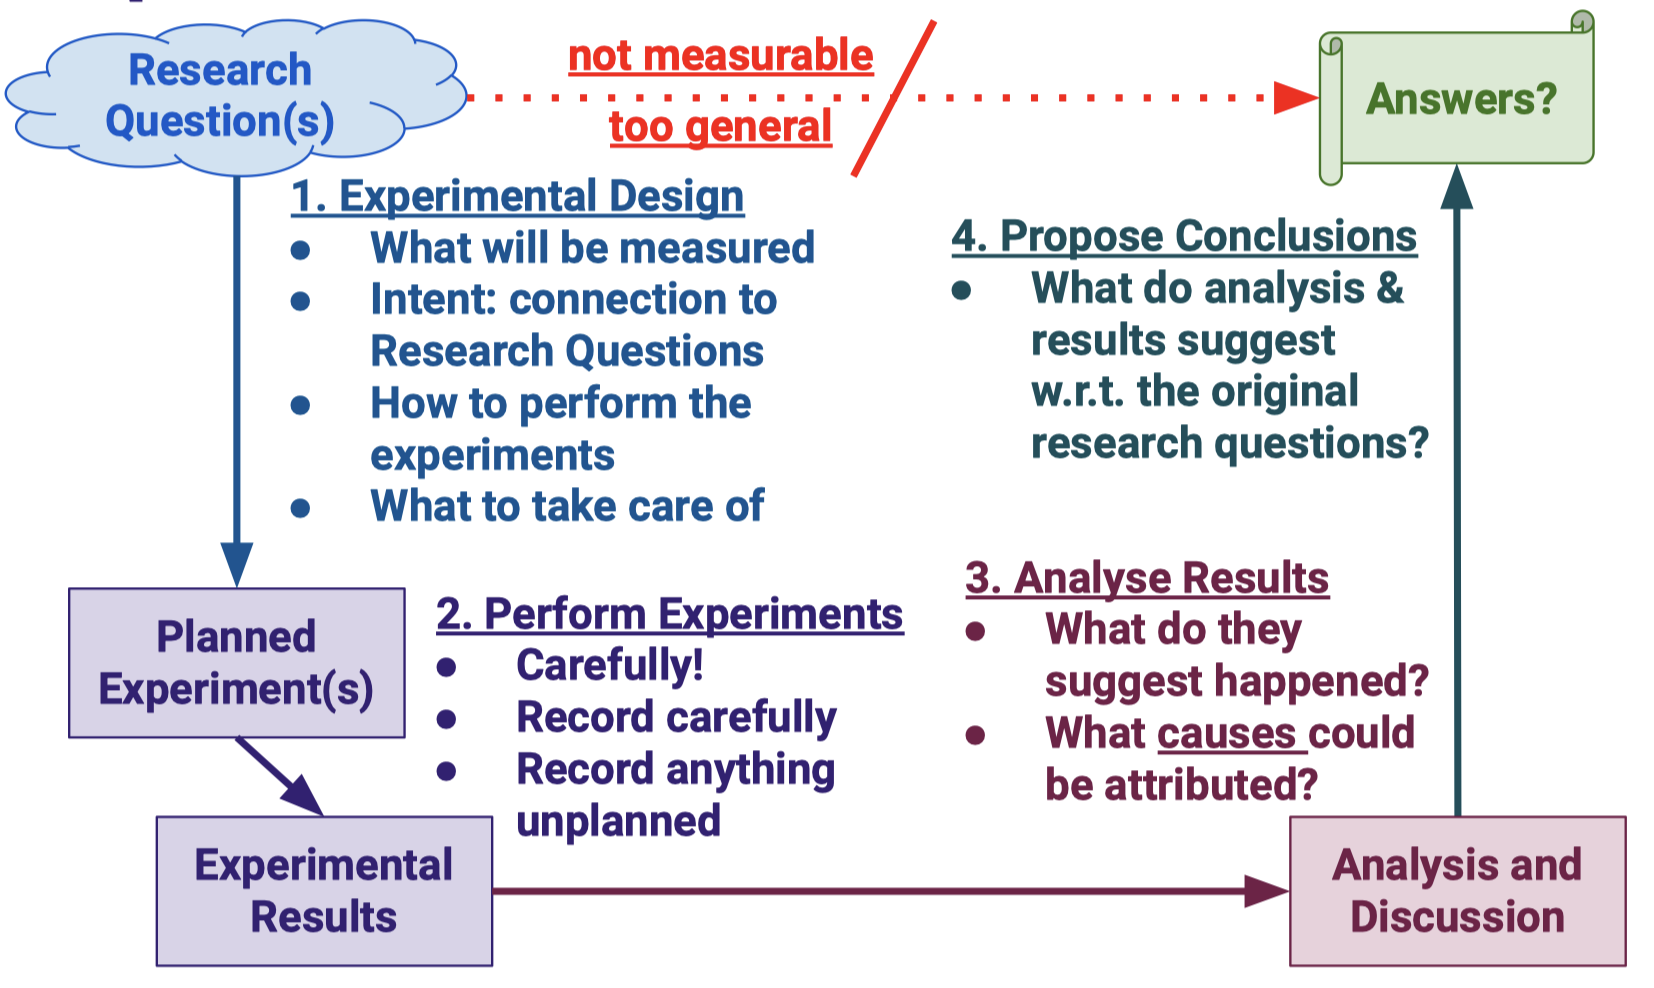
\includegraphics[width=\textwidth]{the_empirical_method}
\end{figure}

\subsection{Threats to Validity}

\begin{itemize}
    \item Construct Validity
    \begin{itemize}
        \item Research Questions $\rightarrow$ Planned Experiments(s)
        \item Are we testing what we mean to test?
    \end{itemize}
    \item Internal Validity
    \begin{itemize}
        \item Experimental Results $\rightarrow$ Analysis and Discussion
        \item Are the results solely due to our manipulations?
    \end{itemize}
    \item External Validity
    \begin{itemize}
        \item Analysis and Discussion $\rightarrow$ Answers?
        \item Are our conclusions justified in general?
    \end{itemize}
\end{itemize}

\section{Program Analysis and Visualization}

\subsection{Main Types of Program Analysis}

\begin{itemize}
    \item Raw Data Analysis
    \begin{itemize}
        \item Analysis of raw data, not structured program representation (e.g. ASTs).
        \item Strengths
        \begin{itemize}
            \item Quick and easy.
            \item Can be built on a pre-exiting raw data analysis.
        \end{itemize}
        \item Weaknesses
        \begin{itemize}
            \item Not precise/detailed.
        \end{itemize}
        \item Applications
        \begin{itemize}
            \item diff
            \item grep, sed
            \item git (e.g. git blame)
            \item Issue tracker info (e.g. GitHub)
        \end{itemize}
    \end{itemize}
    \item Meta-Properties Analysis
    \begin{itemize}
        \item Analysis of project-level/software process metrics.
        \item Applications
        \begin{itemize}
            \item Show git history.
        \end{itemize}
    \end{itemize}
    \item Static Program Analysis
    \begin{itemize}
        \item Analysis of structured source code (ASTs) before running it.
        \item Applications
        \begin{itemize}
            \item Enforcing coding guidelines (value-agnostic).
            \item Reporting potential behaviours (value-sensitive).
        \end{itemize}
    \end{itemize}
    \item Dynamic Program Analysis
    \begin{itemize}
        \item Analysis of code while running it.
        \item Applications
        \begin{itemize}
            \item Runtime checks (e.g. array bounds).
            \item Debugger.
        \end{itemize}
    \end{itemize}
\end{itemize}

\subsection{High-Level Implementation Strategies for Large-Scale Analyses}

\begin{itemize}
    \item Visitor Pattern
    \begin{itemize}
        \item Usage of features from classes.
        \item Indirect dependencies (e.g. subclassing, inherited code)
    \end{itemize}
    \item Existing libraries for exploring Java ASTs
    \begin{itemize}
        \item Eclipse's Java ASTVisitor
        \item javax.lang.model
    \end{itemize}
    \item Frameworks for specifying program analyses declaratively (e.g. Datalog)
    \begin{itemize}
        \item Data extraction: reusable database of facts.
        \item Relations of interest.
    \end{itemize}
\end{itemize}

\subsection{Main Properties About Code}

\begin{itemize}
    \item How the code is written
    \begin{itemize}
        \item Suitable for static analysis.
        \item Examples
        \begin{itemize}
            \item Coding style
            \item Recognising syntactic patterns
        \end{itemize}
    \end{itemize}
    \item What the code does
    \begin{itemize}
        \item Difficult for static analysis.
        \item Examples
        \begin{itemize}
            \item Can this method throw exceptions?
            \item Will this loop terminate?
        \end{itemize}
    \end{itemize}
    \item What the author intended
    \begin{itemize}
        \item Out of scope for static analysis.
        \item Examples
        \begin{itemize}
            \item Under what conditions is calling this function supposed to work?
            \item What should it do?
        \end{itemize}
    \end{itemize}
\end{itemize}

\subsection{All-Executions and Single-Execution Properties}

\begin{itemize}
    \item All-executions property
    \begin{itemize}
        \item Related to the set of all possible executions.
        \item Examples
        \begin{itemize}
            \item Can the method throw exceptions? $\rightarrow$ Is there any execution which does?
            \item Does this method always terminate? $\rightarrow$ Are all executions terminating?
            \item What does this loop compute in general?
        \end{itemize}
    \end{itemize}
    \item Single-execution property
    \begin{itemize}
        \item Related to a single execution.
        \item Examples
        \begin{itemize}
            \item What does this loop compute given one specific input state?
        \end{itemize}
    \end{itemize}
\end{itemize}

\subsection{Static Program Slicing}

\begin{itemize}
    \item Key idea: compute a map before/after each statement from variables to a set of line numbers, representing those the current value of that variable may have been influenced by.
    \item Examples
    \begin{itemize}
        \item L12 (18)
        \item L12 (19-20)
        \item L13 (4-17)
        \item A5 (1)
    \end{itemize}
\end{itemize}

\subsection{Instrumentation}

\begin{itemize}
    \item Instrumenting source code
    \begin{itemize}
        \item Requires less knowledge.
    \end{itemize}
    \item Instrumenting executable
    \begin{itemize}
        \item Applies to other languages that target the same representation.
    \end{itemize}
    \item Online dynamic analysis: run the analysis as part of/alongside the program.
    \begin{itemize}
        \item Influences the execution (e.g. debugger, runtime checks).
    \end{itemize}
    \item Offline dynamic analysis: make the program produce a log, then analyse it separately.
    \begin{itemize}
        \item Simple to implement.
        \item More efficient (but logging may still be expensive).
    \end{itemize}
\end{itemize}

\subsection{Dynamic Program Slicing}

\begin{itemize}
    \item Process
    \begin{itemize}
        \item Create a map (variables to sets of line numbers).
        \item Update the map for every assignment statement.
        \item For branch/loop conditions
        \begin{itemize}
            \item Track a set of line numbers that represent the branch condition(s).
            \item Union these sets when assigning a variable.
            \item No changes to the map at the heads of loops/end of if-then-else.
        \end{itemize}
    \end{itemize}
    \item Examples
    \begin{itemize}
        \item L13 (24)
        \item L13 (25-26)
        \item A5 (3)
    \end{itemize}
\end{itemize}

\subsection{Static vs. Dynamic Slicing}

\begin{itemize}
    \item Static Slicing
    \begin{itemize}
        \item The slice keeps all statements $\rightarrow$ ever relevant.
        \begin{itemize}
            \item Over-estimation (imprecision due to "maybe" questions).
        \end{itemize}
    \end{itemize}
    \item Dynamic Slicing
    \begin{itemize}
        \item A slice is only relevant for a single execution.
        \begin{itemize}
            \item Different input states $\rightarrow$ different behaviours.
            \item Cannot be generalized.
            \item When to stop?
        \end{itemize}
    \end{itemize}
\end{itemize}

\subsection{Over- and Under-Approximations}

\begin{itemize}
    \item Over-approximation: track at least the actual behaviours, but maybe more (e.g. static program slicing).
    \begin{itemize}
        \item Including errors that never happen (false positive).
        \item Including behaviours that the program never actually exhibits.
    \end{itemize}
    \item Under-approximation: track at most the actual behaviours, but maybe less (e.g. only definite dependencies).
    \begin{itemize}
        \item Missing errors that can actually happen (false negative).
        \item Missing behaviours that the program can actually exhibit.
    \end{itemize}
\end{itemize}

\subsection{Satisfiability}

\begin{itemize}
    \item Satisfiability problem: given a set of constraints with unknowns, do there exist values for the unknowns satisfying all constraints?
    \item Examples
    \begin{itemize}
        \item L14 (13-21)
    \end{itemize}
\end{itemize}

\subsection{Symbolic Execution}

\begin{itemize}
    \item A technique for exploring sets of program executions all at once.
    \begin{itemize}
        \item Symbolic values: names that represent values we don't know statically (e.g. $U$, $V$).
        \item Symbolic expression: expression over symbolic values, constants, and operators (e.g. $U < V + 1$).
        \item Symbolic state: mapping from program variables to symbolic expressions (e.g. ($a \rightarrow U$, $b \rightarrow U + 2$)).
        \item Symbolic evaluation of a program expression in a symbolic state $\rightarrow$ symbolic expression
        \begin{itemize}
            \item e.g. $a + b + 7$ and ($a \rightarrow U$, $b \rightarrow U + 2$) $\rightarrow$ $U + (U + 2) + 7$ ($= 2U + 9$)
        \end{itemize}
    \end{itemize}
    \item Examples
    \begin{itemize}
        \item L14 (26)
        \item L14 (27-28)
        \item L14 (29-32)
    \end{itemize}
\end{itemize}

\subsection{Remaining Pain Points}

\begin{itemize}
    \item Indefinitely many initial states/executions
    \begin{itemize}
        \item A (terminating) analysis can't precisely explore them all.
        \item Can ba addressed by symbolic execution.
    \end{itemize}
    \item Branch conditions
    \begin{itemize}
        \item Value-dependent alternative control flow paths.
        \item Can be addressed by symbolic execution.
    \end{itemize}
    \item Loop/recursion
    \begin{itemize}
        \item Unboundedly many control flow paths.
        \item Needs either over- or under-approximation.
    \end{itemize}
    \item Alias information/side effects
    \begin{itemize}
        \item Precisely tracking what changes per assignment/call.
        \item Complex symbolic states.
        \item Needs specialized static analyses.
    \end{itemize}
    \item Dynamically-determined program code
    \begin{itemize}
        \item Dynamic dispatch, reflection.
        \item Needs specialized static analyses.
    \end{itemize}
    \item Concurrency
    \begin{itemize}
        \item Race conditions, non-determination.
        \item Needs specialized static analyses.
    \end{itemize}
\end{itemize}

\section{Digesting and Evaluating PL/SE Research Papers}

\subsection{Key Points of Skim-Reading}

\begin{itemize}
    \item Problem Statement and Motivation
    \begin{itemize}
        \item What is the problem/point?
        \item Where to look
        \begin{itemize}
            \item Title.
            \item Abstract.
            \item Start of the intro.
        \end{itemize}
    \end{itemize}
    \item Claimed Contributions
    \begin{itemize}
        \item What is the claimed value of the paper?
        \item Where to look
        \begin{itemize}
            \item Abstract.
            \item Intro.
            \item Conclusions.
        \end{itemize}
    \end{itemize}
    \item The Approach
    \begin{itemize}
        \item The high level solution/idea behind their solution/approach.
        \item Where to look
        \begin{itemize}
            \item Motivating example
            \item Overview figure
            \item ``Approach''/``Methodology'' section
            \begin{itemize}
                \item Overview
                \item Subsection and figure titles
            \end{itemize}
        \end{itemize}
    \end{itemize}
    \item Evidence Provided
    \begin{itemize}
        \item What evidence is provided to substantiate their claims.
        \item Where to look
        \begin{itemize}
            \item ``Implementation''/``Experimental Evaluation'' section
            \item Tables, graphs, and their captions
        \end{itemize}
    \end{itemize}
    \item High-Level Evaluation
    \begin{itemize}
        \item Conclusions? Comparisons with relevant work? Limitations/weaknesses?
        \item Where to look
        \begin{itemize}
            \item ``Discussion''/``Conclusions'' section
            \item ``Future Work'' section
        \end{itemize}
    \end{itemize}
    \item Research Context
    \begin{itemize}
        \item Citations and references.
    \end{itemize}
\end{itemize}

\end{document}
